\begin{theo}{\textsc{Weierstrass}}
    Toute fonction continue sur un segment $[a, b]$ de $\R$ à valeurs dans $\R$ ou $\C$ est limite uniforme sur $[a, b]$ d'une suite de polynômes.
\end{theo}

\url{https://bibmath.net/dico/index.php?action=affiche&quoi=./w/weierstrass.html} Autrement dit, pour toute fonction $f : [a, b] \to \R$ continue et pour tout $\varepsilon > 0$, il existe un polynôme $P$ tel que
$$\forall x \in [a, b], |f(x) - P(x)| < \varepsilon.$$
Ce théorème affirme que l'ensemble des fonctions polynomiales est dense dans l'ensemble des fonctions réelles continues sur un segment (pour la topologie de la convergence uniforme).

\begin{preuve}
    \marginnote[0cm]{\cite{calcul_infinitesimal} page 157}
\end{preuve} 

\begin{exercice}
    \marginnote[0cm]{fic00042}
    Soit $f \in \mathscr{C}([a, b], \R)$ telle que
    $$\forall n \in \N, \int_a^b f(t) t^n \d t = 0.$$
    Montrer que $f$ est la fonction nulle.
\end{exercice}

\begin{solution}

\end{solution}

L'exercice suivant explicite une suite de polynômes $(P_n)$ qui converge uniformément vers la fonction racine carrée sur $[0, 1]$.

\begin{exercice}
    \marginnote[0cm]{Exercice 5. TD Ch. VIII}
    Soit la suite de fonctions définie pour tout $x \in [0, 1]$ par
    $$
    \begin{cases}
        P_0(x) &= 0,\\
        P_{n+1}(x) &= P_n (x) + \frac{1}{2} \big( x-P_n (x)^2 \big).
    \end{cases}
    $$
    Montrer que $(P_n)$ converge uniformément vers une fonction $f$ sur $[0, 1]$.
\end{exercice}

\underline{Questions intermédiaires:} \\
\begin{enumerate}
    \item Montrer que $(P_n)$ est une suite de restrictions de polynômes dont on précisera le dégré.
    \item Montrer que cette suite converge simplement vers une fonction $f$ à préciser.
    \item Montrer que, pour tout $x \in [0, 1]$ et pour tout $n \in \N$,
    $$0 \leqslant f(x) - P_n(x) \leqslant 2 \frac{f(x)}{2 + nf(x)}.$$
    \item Montrer que $(P_n)$ converge uniformément vers la fonction $f$ sur $[0, 1]$.
\end{enumerate}

\begin{solution}
    Soient $x \in [0, 1]$ et $n \in \N$.
    \begin{align*}
        \sqrt{x} - P_{n+1}(x) &= \sqrt{x} - P_n(x) - \frac{1}{2} \big( x - P_n(x)^2  \big) \\
        &= \big(\sqrt{x} - P_n(x) \big) \left( 1 - \frac{1}{2} \frac{x - P_n(x)^2}{\sqrt{x} - P_n(x)} \right) \\
        \sqrt{x} - P_{n+1}(x) &= \big(\sqrt{x} - P_n(x) \big) \left(1 - \frac{\sqrt{x} + P_n(x)}{2} \right).
    \end{align*}
    Pour tout $n \in \N$ on pose
    \begin{center}
        $\mathscr{P}_n$: \say{ \forall x \in [0, 1], 0 \leqslant \sqrt{x} - P_n(x) \leqslant \sqrt{x} \left( 1 - \frac{\sqrt{x}}{2}  \right)^n }.
    \end{center}
    \begin{itemize}
        \item[$\rhd$] Initialisation pour $n = 0$: immédiat.
        \item[$\rhd$] Hérédité: soit $n \geqslant 0$, on suppose $\mathscr{P}_n$ vraie. \\
        Soit $x \in [0, 1]$, d'après le résultat précédent et l'hypothèse de récurrence,
        \begin{align*}
            0 \leqslant \sqrt{x} - P_{n+1}(x) \leqslant \sqrt{x} \left( 1 - \frac{\sqrt{x}}{2}  \right)^n \times \left(1 - \frac{\sqrt{x} + P_n(x)}{2} \right)
        \end{align*}
        Comme le polynôme $P_n$ est positif, le second terme est majoré par $1 - \frac{\sqrt{x}}{2}$ et donc $\mathscr{P}_{n+1}$ est vérifiée.
    \end{itemize}
\end{solution}

\begin{marginfigure}[-5cm]
    \centering
	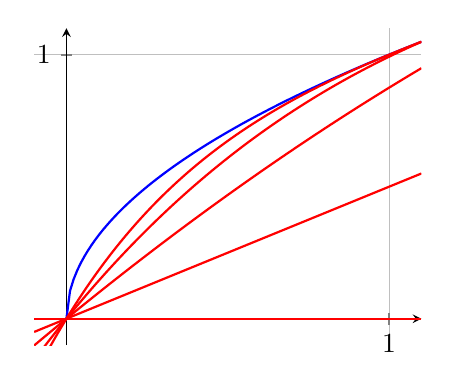
\begin{tikzpicture}
    \begin{axis}[width=6.5cm,
        axis lines=middle,
        grid=major,
        xmin=-0.1, xmax=1.1,
        ymin=-0.1, ymax=1.1,
        % xlabel=$x$, xlabel style={right},
        % ylabel=$y$, ylabel style={above},
        tick style={thick},
        ticklabel style={font=\normalsize},
        xtick={0, 1}, 
        ytick={0, 1},
        % legend entries={0.5x},
            legend style={
            at={(1.05,0.4)},
            anchor=north,
            legend columns=1},
            legend cell align={left}
    ]
    
    \def\a{-0.1}
    \def\b{1.1}
    
    \addplot[blue,thick,samples=100,domain=0:\b] {x^(1/2)} node (racine) {};
    %\node [left] at (racine) {$\sqrt{x}$};
    
    \addplot[red,thick,samples=100,domain=\a:\b] {0} node (P0) {};
    %\node [left] at (P0) {$P_0$};
    
    \addplot[red,thick,samples=100,domain=\a:\b] {x/2} node (P1) {};
    %\node [anchor=north east] at (P1) {$P_1$};
    
    \addplot[red,thick,samples=100,domain=\a:\b] {-1/8*x^2+x} node (P2) {};
    %\node [left] at (P2) {$P_2$};
    
    \addplot[red,thick,samples=100,domain=\a:\b] {-1/128*x^4+1/8*x^3-5/8*x^2+3/2*x} node (P3) {};
    %s\node [left] at (P3) {$P_3$};
    
    \addplot[red,thick,samples=100,domain=\a:\b] {-1/128*x^4+1/8*x^3-5/8*x^2+3/2*x + 1/2*(x-(-1/128*x^4+1/8*x^3-5/8*x^2+3/2*x)^2)} node (P4) {};
    \end{axis}
\end{tikzpicture}


%import matplotlib.pyplot as plt
%import numpy as np
%from numpy.polynomial import Polynomial

%PAS = 1e-3
%n = 8
%X = np.arange(0, 1, PAS)


%P = Polynomial([0])
%plt.plot(X, P(X))

%for k in range(n):
%    P = P + 1/2 * (Polynomial([0, 1]) - P ** 2)
%    plt.plot(X, P(X))

%racine = [np.sqrt(x) for x in X]
%plt.plot(X, racine, 'r')
%plt.show()

	\caption*{\centering Convergence uniforme de la suite $(P_n)$ vers la fonction racine carrée sur $[0,1]$}
\end{marginfigure}

Une question naturelle est de se demander si ce théorème d'approximation peut se généraliser à $\R$. La réponse est non.

\begin{prop}{}
    Si $(P_n)_{n \in \N}$ est une suite de polynômes convergeant uniformément sur $\R$ vers une fonction $f$, alors $f$ est un polynôme.
\end{prop}

\begin{preuve}
    \marginnote[0cm]{\cite{exos_oraux} \& \cite{maths-france}}
    Soit $(P_n)_{n \in \N}$ une suite de polynômes convergeant uniformément sur $\R$ vers une fonction $f$. \\
    D'après la critère de \textsc{Cauchy} uniforme, il existe un rang $n$ tel que pour tout $p \in \N$, 
    $$\Ninf{P_{n+p} - P_n} \leqslant 1.$$
    La fonction polynomiale $P_{n+p} - P_n$ est donc bornée sur $\R$ autrement dit elle est constante. On a alors,
    $$\forall (p, x) \in \N \times \R,\ P_{n+p}(x) = P_n(x) + P_{n+p}(0) - P_n(0) \xrightarrow[p \to + \infty]{} P_n(x) + f(0) - P_n(0)$$
    donc par unicité de la limite simple, $f : x \mapsto P_n(x) + f(0) - P_n(0)$, qui définit bien une fonction polynomiale. 
\end{preuve}